\documentclass[12pt]{article}
\usepackage{hyperref}
\usepackage{amsmath, amssymb, amsfonts}
\usepackage[margin=1.2cm]{geometry}
\usepackage{xcolor}
\usepackage{graphicx}
\usepackage{enumitem, inconsolata}
\usepackage{tikz}
\usepackage{circuitikz}[scale=1.2]
\usetikzlibrary{patterns}
\parindent 0px
\newcommand{\W}{\(\Omega\)}
\newcommand{\w}{\(\omega\)}
\newcommand{\lb}{\\$\left|\rightarrow\right.$}
\newcommand{\enter}{\\\textcolor{white}{1}}
\newcommand{\sub}[1]{\textsubscript{#1}}
\newcommand{\super}[1]{\textsuperscript{#1}}
\ExplSyntaxOn
\NewDocumentCommand{\bo}{m}
 {
   \bold_commas:n { #1 }
 }

\cs_new:Npn \bold_commas:n #1
 {
   \seq_set_split:Nnn \l_tmpa_seq { , } { #1 }
   \seq_map_indexed_function:NN \l_tmpa_seq \__bold_commas_aux:nn
 }

\cs_new:Npn \__bold_commas_aux:nn #1 #2
 {
   \textbf{#2}
   \int_compare:nNnTF { #1 } < { \seq_count:N \l_tmpa_seq }
     { , }
     { }
 }

\ExplSyntaxOff

\title{Object Oriented Software Engineering}
\author{by PUL079BEI008}
\date{\today}

\begin{document}
\maketitle
\vspace{8.5cm}
\textbf{Notes}
\begin{itemize}[noitemsep]
	\item Our subject code is CT 659.
	\item This document encorporates for both, electronics and computer department's Object Oriented Analysis and Design (CT 651).
	\item If a question was asked in Regular Exam, it is kept in \bo{boldened} form. If it was asked in back exam, it is in regular font.
  \item If its electronic's paper, then it \texttt{will be marked with this font}, if OODE's, then it will be normal font.
	\item Months are marked as: 
	\begin{itemize}[noitemsep, topsep=0pt]
		\item Ba: Baisakh
		\item Jth: Jestha
		\item Asa: Ashar
		\item Shr: Shrawan
		\item Bh: Bhadra
		\item Ash: Ashwin
		\item Ka: Kartik
		\item Mng: Mangsir
		\item Po: Poush
		\item Ma: Magh
		\item Ch: Chaitra
	\end{itemize}
\end{itemize}
\pagebreak
\tableofcontents
\pagebreak

\section{Introduction to Software and Software Engineering}
  \begin{center} (5 Hours / 8 Marks) \end{center}
 
  \subsection{Introduction to software engineering}
    \begin{enumerate}
      \item Elaborate the meaning and need of Software Engineering. \hfill [2] (\bo{\texttt{78 Ch}})

      \item Differentiate between functional and non-functional requirements. \hfill [3] (\bo{\texttt{81 Ch, 78 Ch}}) [5] (\bo{80 Ch, 79 Ch})
        \lb Explain functional and non-functional requirements with proper example of each. \hfill [4] (\texttt{79 Ash}) [3+3] (75 Ba)
    \end{enumerate}

  \subsection{Software processes and software process models}
    \begin{enumerate}
      \item Define Software Process. \hfill [1] (\bo{\texttt{80 Ch}})

      \item Explain SDLS in the context of OOAD/OOSE. \hfill [5] (\bo{81 Ch})

      \item Explain the general activities involved in software process. \hfill [2] (\bo{\texttt{80 Ch}})

      \item Explain the importance of modern age software engineering. \hfill [3] (\bo{\texttt{81 Ch}})

      \item Justify this statement ``Walking on water and developing software from specification are easy if both are frozen". \hfill [5] (\bo{\texttt{80 Ch}})

      \item Explain waterfall process model with its pros and cons. \hfill [5] (\texttt{82 Ka})

      \item Explain about prototyping process model
        \lb highlighting its importances in software development. \hfill [5] (\bo{\texttt{81 Ch}})
        \lb with its pros and cons. \hfill [5] (\texttt{80 Ash})

      \item Explain iterative development in OOSE. \hfill [4] (\bo{\texttt{81 Ch, 79 Ch, 78 Ch}})

      \item As the Team Lead of a software development team employing iterative development for a project, provide a concise overview of how the iterative process works. Identify its key benefit and a potential drawback. \hfill [5] (\bo{\texttt{80 Ch}})

      \item Explain the Spiral Life cycle model with its adv and disadv. \hfill [6] (\bo{\texttt{79 Ch}})

      \item How do you differentitate classical and modified waterfall lifecycle model? \hfill [2] (\bo{\texttt{78 Ch}})
    \end{enumerate}

  \subsection{Agile Software developments}
    \begin{enumerate}
      \item What is iterative development model? \hfill [4] (\texttt{82 Ka})

      \item Write short ntoes on: Agile Software Development. \hfill [4] (\bo{\texttt{78 Ch}})
        \lb Write short notes on: Agile Method. \hfill [3] (\bo{74 Bh})

      \item What are the strengths of the agile development method? \hfill [2] (75 Ba)
    \end{enumerate}

  \subsection{Requirements engineering processes}
    \begin{enumerate}
      \item Explain requirement engineering process in software development. \hfill [5] (\bo{\texttt{81 Ch, 80 Ch}, 80 Ash}) [6] (\bo{\texttt{79 Ch}})
        \lb Define. \hfill [1] (\bo{78 Ch})

      \item What are the major activities of requirement engineering process? \hfill [4] (\texttt{79 Ash})

      \item What is requirement gathering? \hfill [1] (\bo{80 Ch})

      \item Why do we need to understand the requirements in a different way, how do the requierments are analyzed by different stakeholders? \hfill [3] (\texttt{82 Ka})

      \item Is requirement analysis the same ofr every software development process? Justify your answer. \hfill [5] (\texttt{82 Ka})

      \item Why we need to identify the requirement while developing object-oriented software engineering? \hfill [3] (\bo{\texttt{81 Ch}})
    \end{enumerate}  

  \subsection{System Modeling}
    \begin{enumerate}
      \item Why do we need different types of system models while developing any system? \hfill [2] (\bo{77 Ch})
    \end{enumerate}

  \subsection{Software prototyping}
  \subsection{Object oriented software development}

\pagebreak

\section{Object Oriented Concepts and Modeling}
  \begin{center} (8 Hours / 15 Marks) \end{center}

  \subsection{Introduction to class, object, inheritance, polymorphism}
    \begin{enumerate}
      \item Write short notes on: Inheritance and Polymorphosim. \hfill [4] (\texttt{80 Ash})
    \end{enumerate}

  \subsection{Object oriented system development}
    \subsubsection{Object Oriented Modeling}
      \begin{enumerate}
        \item Explain object-oriented concepts with suitable examples. \hfill [4] (\texttt{82 Ka})
        \lb What are the major concepts of object orientation? \hfill [2] (\texttt{79 Ash})

        \item Explain object oriented system development process. \hfill [5] (75 Ba)

        \item Explain and illustrate the fundamental concepts of object orientation. \hfill [4] (\bo{77 Ch})

        \item What are the benefits of object orientation? \hfill [4] (\texttt{79 Ash})
          \lb What are the advantage of object oriented system over function oriented system? \hfill [2] (\bo{80 Ch})
          \lb What are advantages of OOS over procedural system? \hfill [2] (\bo{75 Bh})

        \item What are the differences of OO based system to other conventional design in context with encapsulation and inheritance? \hfill [4] (\bo{78 Ch})
          \lb Compare between function oriented and object oriented system. \hfill [2] (\bo{78 Ch})

        \item What are the meaning of object and encapsulation in terms of OOAD? Explain briefly with example. \hfill [6] (\bo{74 Bh})

        \item What are the main differences of OO based design cycle to other conventional design cycle? Explain with relevant example. \hfill [6] (75 Ba)

        \item What is the key difference between conventional design approaches to modern OO design cycle? Explain with relevant examples. \hfill [6] (\bo{77 Ch})

        \item Write short notes on: CRC in object modeling. \hfill [4] (\texttt{79 Ash})
          \lb Write short notes on: CRC Cards. \hfill [3] (\bo{81 Ch, 79 Ch}, 73 Ma) [4] (\bo{78 Ch, 76 Bh})
          \lb Write short notes on: CRC Cards and importance in object modeling. \hfill [5] (\bo{77 Ch})

        \item What is the purpose of CRC Cards as a tool for analysis? \hfill [2] (\bo{74 Bh}) [4] (\bo{80 Ch})
      \end{enumerate}

    \subsubsection{Object Oriented System}
      \begin{enumerate}
        \item Describe the term OOA, OOD, and OOP. \hfill [4] (\bo{76 Bh})
      \end{enumerate}


    \subsubsection{Function/data Methods}
      \begin{enumerate}
        \item Compare Function and Data Method with Object Oriented Approaches. \hfill [4] (\bo{\texttt{81 Ch}, 82 Ka, 80 Ash})

        \item What are the differences between function/data methods and object-oriented methods for system development? \hfill [3] (\bo{\texttt{78 Ch}})
      \end{enumerate}
    
    \subsubsection{Object Oriented Analysis}
      \begin{enumerate}
        \item Explain how the requirement elicitation process happens in OOA. \hfill [4] (75 Ba)
      \end{enumerate}

    \subsubsection{Object Oriented Programming}

    \subsubsection{Object Oriented Construction}

  \subsection{Identifying the elements of an object model}
    \subsubsection{Identifying classes and objects}
      \begin{enumerate}
        \item How is object element is identifying and constructed in object-oriented software development? \hfill [6] (\bo{\texttt{80 Ch}})

        \item How can we identify objects in a system? Explain with appropriate examples. \hfill [5] (\bo{\texttt{79 Ch}})

        \item How can we identify potential classes and object of an object model? Explain with an example. \hfill [4] (\texttt{80 Ash}) [5] (\bo{\texttt{78 Ch}})
      \end{enumerate}

    \subsubsection{Specifying the attributes}
      \begin{enumerate}
        \item (Assumed) Explain attribute, paramter and global visibility with an example. \hfill [6] (\bo{80 Ch})

        \item (Assumed) Discuss the visiblity as per the OOD with example. \hfill [5] (\bo{79 Ch})

        \item (Assumed) What is attribute and parameter visibility? \hfill [2] (\bo{78 Ch})

        \item (Assumed) Write short notes on: Association visibility. \hfill [3] (\bo{74 Bh}) 
      \end{enumerate}

    \subsubsection{Defining operations}
    \subsubsection{Finalizing the object definition}

\pagebreak

\section{Structural, Behavioral and Architectural Modeling}
  \begin{center}
    (8 Hours / 14 Marks)\\
    Focus more on Class, Use Case, Sequence and Activity Diagram for new syllabus
  \end{center}
 
  \subsection{Classes Relationship}
    \begin{enumerate}
      \item Explain about class relationships with appropriate symbols. \hfill [4] (\texttt{82 Ka})
      \lb Write short notes on: Class Relationship. \hfill [3] (\bo{\texttt{81 Ch}}) [4] (\bo{\texttt{79 Ch, 78 Ch}, 80 Ash})
    \end{enumerate}

  \subsection{Conceptual Model of UML}
    \begin{enumerate}
      \item Explain conceptual model of UML. \hfill [4] (\texttt{80 Ash})

      \item (Assumed) Write short notes on: Conceptual model and Implementation. \hfill [4] (\bo{80 Ch})
        \lb on: Conceptual model vs Implementation model. \hfill [4] (\bo{78 Ch})

      \item What are the perceptions of applying UML? \hfill [2] (\bo{74 Bh})

      \item Write short notes on: Pros and Cons of UML/OMT use in system development. \hfill [4] (76 Ba)

      \item Write short notes on: Behavioral model of the system. \hfill [4] (76 Ba)

      \item In OOAD, there are various types of models, like conceptual, structural, behavioral, etc. What is the significance of these many different types of model? Explain with illustrative examples. \hfill [6] (\bo{74 Bh})

      \item Explain the basic building blocks of the UML. \hfill [4] (\bo{\texttt{80 Ch}}, \texttt{79 Ash}) [6] (\bo{77 Ch})

      \item Why do we need UML is software development? \hfill [2] (\bo{\texttt{81 Ch}})

      \item How can you express exceptions in UML diagrams? Illustrate with possible exceptions in any suitable scenario. \hfill [6] (\bo{75 Bh})

      \item Justify the statement ``The UML is a language for Visualizing, Specifying, Constructing and Documenting the artifacts of a software-intensive system." \hfill [4] (\bo{\texttt{80 Ch, 78 Ch}}, 76 Ba)

      \item What are the elements of the Conceptual Model of UML? Explain. \hfill [4] (\bo{\texttt{79 Ch}})

     
      \item Explain primary relationship between class, dependency, association, aggregation and composition with their corresponding nation. \hfill [6] (75 Ba)

      \item Write short notes on: Adornment of relation. \hfill [3] (7 Ma)

      \item What are the various types of UML diagrams drawn to handle static and dynamic conponent of software under development? \hfill [3] (\texttt{79 Ash})

      \item Write short notes on: Five views of UML. \hfill [3] (\bo{81 Ch})

      \item Explain dependency, aggregation and composition with proper symbols. \hfill [6] (\bo{81 Ch})
        \lb explain association \textit{instead of dependency}. \hfill [6] (\bo{75 Bh})
        \lb also association with notation and example. \hfill [7] (\bo{80 Ch})
        \lb also association with example. \hfill [4] (\bo{78 Ch})
        \lb also generalization with notation and example. \hfill [6] (\bo{79 Ch})

      \item Describe the methods to find out the conceptual classes. \hfill [2] (\bo{76 Bh}) [3] (76 Ba)
        \lb How do you find candidate conceptual classes of a system using category list method? Explain with example. \hfill [5] (\bo{79 Ch})

      \item What do you mean by conceptual classes? \hfill [1] (\bo{76 Bh}, 75 Ba)

      \item Define Domain modeling. \hfill [2] (75 Ba) [6] (\bo{78 Ch})
        \lb with its necessary components. \hfill [2] (\bo{77 Ch})

      \item How domain model lowers representational gap between conceptual and software model?\hfill [3] (76 Ba)

      \item List out the steps to draw domain model and describe each step. \hfill [2] (\bo{77 Ch})

      \item Construct domain model with respect to outlined steps for the following case study. \hfill [6] (\bo{77 Ch})\\
        Patients are treated in a single ward by the doctors assigned to them. Healthcare assistants also attend to the patients, a number of these are associated with each ward. Each patient is required to take a variety of drugs a certain number of times per day and for varying lengths of time. The system must record details concerning patient treatment and staff payment. Some staffs are paid part time and doctors healthcare assistants work varying amounts of overtime at varying rates. The system will also need to track what treatments are required for which patients. \hfill [6] (\bo{77 Ch})

      \item Identify the conceptual classes and its supportive attributes for given scenario and draw domain model for the system. \hfill [7] (\bo{80 Ch})\\
        A customer arrived at the checkout counter with items to purchase. The cashier uses the POS system to record each item. This system presents running total and line item details. The customer enters payment information which system validates and records. Then system updates the inventory. The customer receives receipt from the system and elaves the store with the purchased item.

      \item Consider the Library System. Each book in a library contains bibliography, each bibliography consists of a number of reference to other books. A book will be referred to in many cases and therefore a reference can appear in more than one bibliography. Use noun phrase identification strategies to find the conceptual classes of above cases. \hfill [4] (\bo{74 Bh})

      \item List the candidate conceptual class for Online Movie Ticket Booking System by using the Category list method.
        \enter\hfill [4] (\bo{78 Ch})
    \end{enumerate}

  \subsection{Class Diagram}
    \begin{enumerate}
      \item (Assumed) How can we create class definition and methods from the domain class diagram and interaction diagrams? Explain with appropriate example. \hfill [4+4] (73 Ma)

      \item What is the role of constraint specifications in a model diagram? The model below figure depicts about possible types of accounts within the portfolio sub-head in any banking business domain. Identify the constraints highlighted and explain brief, what they mean. Write pseudocode the model diagram. \hfill [8] (\bo{74 Bh})\\
        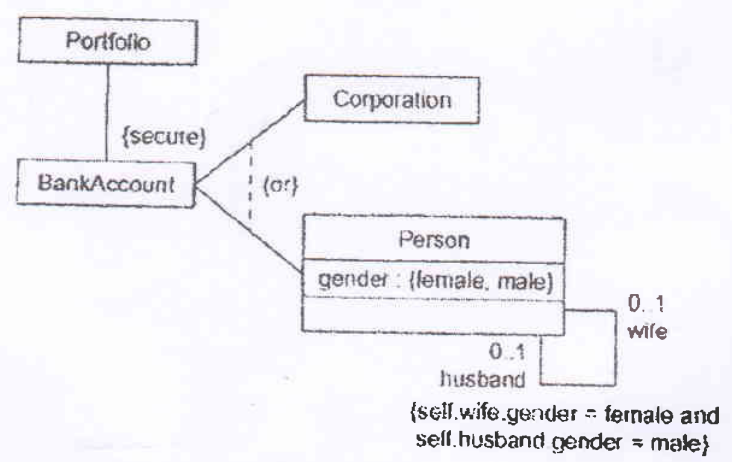
\includegraphics[width=5in]{images/oose_74_bh}

      \item Draw the class diagram for ``Library Management System" \hfill [5] (\texttt{80 Ash})

      \item Draw a class diagram for the Flight Management System with necessary assumptions. \hfill [6] (\bo{\texttt{78 Ch}})

      \item Draw the class diagram of ticket reservation for Kathmandu to Pokhara and vice versa for public bus service. \hfill [6] (\texttt{82 Ka})

      \item For the following case study, identify classes, attributes, methods, relationships between classes and draw class case diagram.\\
        ABC bank has many branches, each of which has an address and branch number. Each branch may have upto three extension counters. A customer opens accounts at a branch. Each account is uniquely identified by an account number; it has a balance and a credit overdraft limit. There are many types of accounts like a saving account. A current acount and a credit account which has an expiry date and can have secondary cards attached to it. It is possible to have a joint account (e.g., for a husband and wife). Each type of account has a particular interest rate, a monthly fee and a specific set of privileges (e.g., ability to write cheques, insurance fr purchase, etc.) ABC bank is divided into divisions and subdivisions (such as Risk Management, Planning, Investmets and Consumer), the branches are considered subdivisions of the consumer division. Each division has a manager and a set of other employees. Each customer is assigned a particular employee as his or her `personal banker'. \hfill [7] (\texttt{79 Ash})

      \item Create a category list for Airline reservation application and explain how you would use it to idenitfy conceptual classes. Construct a class diagram for the following scenarios: \hfill [4+6] (\bo{81 Ch})\\
        For a construction company, a software is to be developed with following specifications: Company takes many projects at particular location. Each project is supervised by project manager assigned by CEO of the company. Record related to start of the project, completion of the project is maintained. Under each project manager, there is a team of people of different category like designer, plumber, electrician, architect, labor, etc. Each project is marketed by a team of marketing executives.

      \item Create a class diagram for an online doctor consultation enabling patients to register, log in, upload and save medical reports. Upon successful completion of the above actions, he/she can engage with doctor for personalized insights. \hfill [6] (\bo{80 Ch})

      \item Identify conceptual class and its supportive attributes for a Photocopier machine from the description given below and draw the conceptual class diagram for the same.
        Initially the machine is off. When the operator switches on the machine, it first warms up during which it performs some internal tests Once the tests are over, machine is ready for making copies. When operator loads a page to be photocopied and press 'start' button, machine starts making copies according to the number of copies selected. When the machine is making copies, machine may go out of paper. Once operator loads sufficient pages, it can start making copies again. During the photocopy process, if paper jam occurs in the machine, operator may need to clean the path by removing the jammed paper to make the machine ready. \hfill [9] (\bo{74 Bh})

      \item Identify the different classes, relationships and draw a class diagram for ``Online Examination System" as the following: \hfill [8] (\bo{78 Ch})\\
        Students can login to the system with the username and password provided to them. Students can be new or existing. Student can register for the exam through the online form provided in the system. Students are requested to pay for the examination after the registration of the exam. Payments for the registration are accepted through the Bank. Bank verifies the clearance of fee. Administrator manages the system through faculty id, course code, course slot, create exam, delete exam, update exam and check report. Question paper provided to student through the system. Students can give exam and check report after the exam. \hfill [8] (\bo{78 Ch})

      \item For the case study given below identify all classes, their relationships, attributes and methods for each class. Also draw class diagram using standard UML Notation. \hfill [8] (\bo{75 Bh}) \enter
        Makalu College operates international business in 10 location throughout the globe. The college has its first 9000 graduates in 2010. The second keeps track of each student's name, country of birth, current address. In order to maintain strong ties to its alumni, the school holds various events around the workld. Events have title, date, location and time. The school needs to keep track of which graduates have attended which events. For an attendance by a graduate at an event, a comment is recorded about information. School officials learn from that graduate at that event. As with the events, school records information learned from graduates. When an official knows that he or she will be meeting or talking to graduates. When an official knows that he or she will be meeting or talking to graduate, a report is produced showing the latest information about the graduate and the information learned during the past two years from that graduate from all contacts and events the graduate attended.
    \end{enumerate}

  \subsection{Advanced classes, Advanced Relationship, Interface}
    \begin{enumerate}
      \item Write short notes on: Advanced class. \hfill [4] (\bo{\texttt{80 Ch}})
    \end{enumerate}

  \subsection{Object Diagram}
    \begin{enumerate}
      \item Write short notes on Object diagram. \hfill [3] (\bo{81 Ch, 80 Ch, 79 Ch})
    \end{enumerate}

  \subsection{Use case Concepts}
    \begin{enumerate}
      \item Explain include and extends relationship in use case diagram. \hfill [2] (\bo{81 Ch}, \texttt{79 Ash})
        \lb with suitable diagram. \hfill [3] (\bo{78 Ch})

      \item What are the advanced relationships on Use case diagram? \hfill [2] (\bo{78 Ch})

      \item Prepare the fully labeled use cases for cash withdraw case of the banking system. \hfill [6] (\bo{74 Bh})
    \end{enumerate}

  \subsection{Use Case Diagram}
    \begin{enumerate}
      \item Draw the use case diagram for ``Car Rental System" \hfill [5] (\texttt{80 Ash})

      \item Draw a use case diagram for Online Bus ticketing System with necessary assumptions. You are requested to write a use case scenario for this system with proper format. \hfill [4] (\texttt{82 Ka})

      \item For the case study given below identify all the actors, use cases and relationships, also draw use case diagram.\\
        Software version of Monopoly game.\\
        This will run as a simulation, the user will configure the game (i.e. indicate the number of players, etc.), start the simulation and let the game run to its conclusion. A trace log will be created to record each move a player makes. The simulation should include the rules of the game and keep track of the amounts each plyer earns/loses throughout the game. The simulation should allow the user to select various strategies to be employed by the players in the game. \hfill [5] (\texttt{79 Ash})
      
      \item Identify actors, use-cases and relationships from following scenario and draw the use case diagram.\\
        Ministry of Health and Population is willing to computerize its system. This new system will be able to tell the population of the country, zone and district nad even ward of specific place. The system will update its data in monthly basis so that the birth rate and death rate can be easily seen. The home page is displayed when a person enters to the system. Administrators can enter to the system by loggin in with an ID and a password. He/She has privileges to enter and modify them. They can also visualize the data in graphical form, maps as well as tabular form. Besides, they can also view the forecasted data. \hfill [6] (\bo{81 Ch})

      \item Consider the Railway Reservation System. There are a number of trains and each train stops in one or more. Each train has a predetermined number of seats available in each of classes (First class, First AC, Second AC, Third AC, Sleepr and so on). The fare between two stations is determined by the class of travel and the distance. Passenger can enquire about the availability of seats betweena any two stations and for any class. The Railway Reservation System should be able to handle the queries and perform the encessary reservation/concellation operation. Draw a use case diagram with the relationships. \hfill [8] (\bo{78 Ch})

      \item For the case study given below, identify all the actors, use cases and relationships and draw use case diagram. \hfill [7] (\bo{76 Bh})\\
        Homework assignment and collection are an integral part of any educational system. Today, this task is performed maually. What we want the homework assignment assignment and collection system (HACS) to do is to automate this process. For the above requirement system administrator perform necessary setup, configuration and security management anad user creation related activities in system. HACS can be used by the instructor to distribute the homework assignments, review the students' solutions, distribute the suggested solution, and distribute student grades on each assignment. HACS shall also help the students by automatically distributing the assignments to the students, provide a facility where the students can submit their solutions, remind the students when an assignment is almost due, and remind the students when an assignment is overdue.

      \item Prepare a Use Case diagram for Online Movie Ticket booking system with necessary assumptions. \hfill [6] (\bo{\texttt{78 Ch}})

      \item Consider the scenario of flight booking through an online system at first and then with allowance of certain days of delay for final purchase through second round of payment process completion. Identify all the actors, use-cases and relationship. Also draw use case diagram. \hfill [8] (73 Ma)

      \item Draw a complete UCD and domain model with proper UML notation for the following case study.
        \enter A university registrar's maintains data about the following entities: Courses, inclduing number, title, credits, syllabus and prerequisities; Course offerings, including course number, year, semester, section number, instructor (s), timing and classrooms; Students, including student id, name and program; and instructors, including identification number, name, department, and title. Further the enrollment of students in courses and grades awarded to students in each course they are enrolled for must be appropriately modeled. \hfill [8] (75 Ba)
    \end{enumerate}

  \subsection{Interaction Diagram}
    \begin{enumerate}
      \item What are the differences between a sequence diagram and a collaboration diagram? \hfill [4] (76 Ba)
        \lb How is sequence diagram different from collaboration diagram. \hfill [2] (73 Ma)

      \item Differentiate between Synchronous and Asynchronous messages in a sequence diagram. \hfill [2] (\texttt{82 Ka})

      \item State-sequence diagram aids the implementation of Reactive system. If you agree on statement, justify with reason and model diagram. \hfill [6] (75 Ba)

      \item (Assumed) The model depicts the clone of Instagram as figure below. Explain in detail the diagram type with every symbol being used and semantics of this diagram. \hfill [8] (\bo{78 Ch})\\
      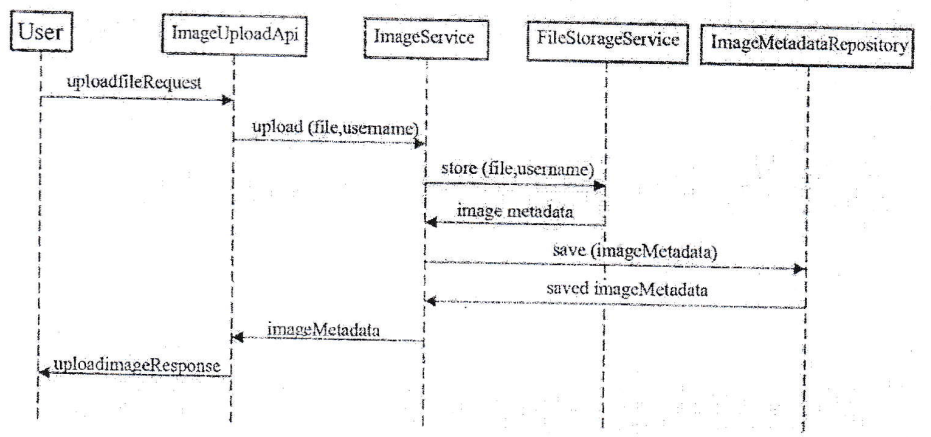
\includegraphics[width=4.3in]{images/oode_78_bh}

      \item Construct a System Sequence Diagram (SSD) for online examination system with necessary assumptions. \hspace{14.7cm} [6] (\bo{75 Bh})

      \item Prepare the sequence diagram of bus ticket reservation system. \hfill [6] (73 Ma)

      \item The model depicts the online order processing system as illustrated below. Explain in detail of the diagram type with every symbols being used and semantics of this diagram. \hfill [8] (75 Ba)\\
      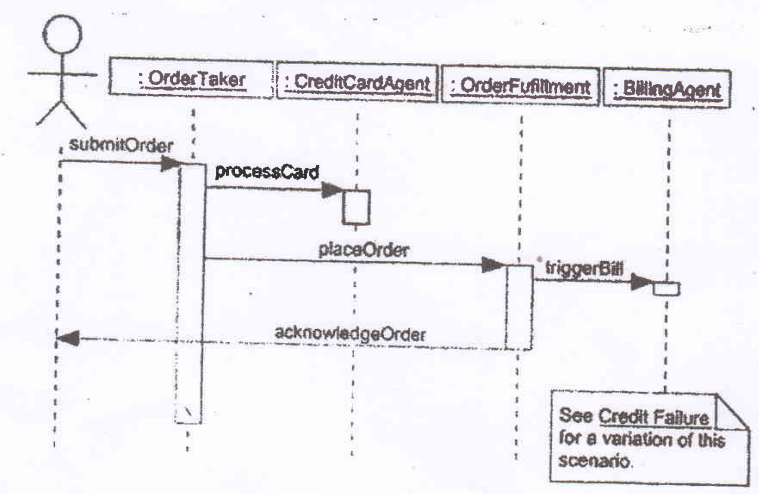
\includegraphics[width=4.3in]{images/oode_75_ba}
    \end{enumerate}

  \subsection{Activity, State Chart, Components, Deployment Diagram}
    \begin{enumerate}
      \item Write short notes on: Swimlanes in activity diagram. \hfill [3] (73 Ma)

      \item Compare: Forking v Joining. \hfill [3] (73 Ma)

      \item Write short notes on: Reactive system and State Chart diagram.  \hfill [4] (\bo{76 Bh})

      \item Draw Activity Diagram for the student enrollment in the university using appropriate symbols:
        \begin{itemize}[noitemsep, topsep=0pt]
          \item An applicant wants to enroll in the university
          \item The applicant hands a filled-out copy of the enrollment form.
          \item The registrar insepcts the forms.
          \item The registrar determines that the forms have been filled out properly.
          \item The registrar informs student to attend a university overview presentation
          \item The registrar helps the student to enroll in seminar
          \item The registrar asks the student to pay for the initial tuition.
        \end{itemize}

      \item Prepare an activity diagram for computing a restaurant bill. There should be a charge for each delivered item. The total amount should be subject to tax. There is a service charge of 18\% for groups of six or more and 10\% for smaller groups. Any coupons and gift certifications submitted by the customer should be subtracted. \hfill [8] (75 Ba)

      \item Prepare the activity diagram for restaurant booking system. \hfill [4] (75 Ba)\\
        (\textit{Yes, 2 separate questions of same type in paper for 75 Ba})

      \item Draw System State Diagram (SSD) and Activity Diagram for the given scenario: \hfill [4+4] (\bo{81 Ch})\\
        Customer arrives at a POS checkout with goods and/or services to purchase. Cashier starts a new sale. Cashier enters item identifier. System records sale line item and presents item description, price and running total. Cashier repeats steps 3-4 until indicates done. System presents total with taxes calculated. Cashier tells Customer the total and asks for payment. Customer pays and System handles payments.

      \item Drawn an Activity Diagram using swim lanes for the scenario given below:\\
        A computer security system has a firewall system and a server that sends the input to the computer. The firewall on the other hand traces the data packet received, source and destination with IP address and port number. There are rules in the firewall to accept or deny the pacekts received. The rules evaluate the validity of the data packets received. After evaluation, the data packets are directed to the concerned application if accepted or discarded if denied. \hfill [8] (\bo{76 Bh})

      \item Write short notes on: Deployment diagram and importance in OO system design. \hfill [5] (\bo{77 Ch})
    \end{enumerate}

  \subsection{Multiple Diagrams}
    \textit{In order/priority of \textbf{Class, Use Case, Sequence, Activity, Deployment}}
    \begin{enumerate}
      \item A library has books, videos and CDs that it loans to its users. All library material has unique id and a title. In addition, books have one or more authors, video have one producer and one or more actors, while CDs have one or more entertainers. The library maintains one or more copies of each library item (book, video or CD). Copies of all library material can be loaned to users. Reference-only material in loaned for 2 hours and can't be removed from library. Other material can be loaned for 2 weeks. For every loan, the library records the user, the loan date and time, and return date and time. For users, the library maintains their name, address and phone number. \hfill [2+4] (\bo{77 Ch})
        \enter a. List out 5 responsibilities from above case and draw \textbf{Interaction diagram} with proper UML notation for any two responsibilities.
        \enter b. Create \textbf{Class diagram} with appropriate association such as aggregation, composition, generalization and dependencies.

      \item Read the following and answer the given questions. \hfill [6x4] (76 Ba)\\
        Customer arrives at the reception of Telephone office to buy a new landline telephone. Receptionist requests to fill up an application form and send him to Sales department. Sales department asks for nearest neighbor's telephone number and search in the Sales Division (SD) System so that SD system displays information including availability of telephone distribution point (DP). If DP is not available, sales department requests customer to submit application form and tells him they will make ocntact if distribution point became available in future. And customer leaves the office. Otherwise, sales officer enters customer details in SD system and sends him to telephone distribution department. Telephone distribution department makes cost estimation and forward him to cash counter for payment. Cashier receives cash and prints and receipt after payment process and send him back to telephone distribution department. Customer presents receipt to telephone distribution department os that telephone distribution department provides/installs new landline telephone service to the customer.
          \enter a. Re-write the above scenario to make it online then: \hfill [5] (76 Ba)
          \enter b. Draw a complete \textbf{Use case} diagram.
          \enter c. Draw a \textbf{Class diagram} showing all the associations, multiplicity, attributes and behaviors.
          \enter d. Draw an \textbf{Activity} diagram.
          \enter e. Convert class diagram \textbf{To code} by using any object oriented programming language of your choice.

        \item Draw \textbf{Class} diagram and \textbf{Activity} diagram with object flow depiction on the following scenario operating condition system:
        Patient can arrange and cancel appointment with physician using scheduler. Physician secceded to prescribe medication for patient. Physician specifies durg info: Medication name, Dosage amount, Number dosages and Refills. Computer cross checks for conflict btween Medication and current Medications/Medicals history prescription forwardd electronically to Pharmacy and printed for patient as well. \hfill [5+5] (73 Ma)

      \item Assume following scenario and draw \textbf{Use case} diagram, \textbf{Sequence} diagram and \textbf{Activity} diagram.\\
        An e-commerce platform allows customers to browse products, add them to their cart, and place orders. Each order may contain multiple products. The system checks product availability before confirming the order. After an order is confirmed, it notifies the warehouse team to prepare the shipment. Customers can view their order status and track the shipment. The system also sends email notifications to customers about order confirmation, payment updates and shipping details.
        \enter\hfill [5+5+5] (\bo{\texttt{81 Ch}})

      \item Develop UML \textbf{Use case} diagram and \textbf{Activity} diagram for the following scenario.
        Sajha Yatayat owns a number of buses. Each bus is allocated to a particular route, although some routes may have several buses. Each route passes through a number of towns. One or more drivers are allocated to each stage of a route, which corresponds to a journey through some or all of the towns on a route. Some of the towns have a garage where buses are kept and each of the buses are identifying by the registration number and can carry different numbers of passengers, since the vehicles vary in size and can be single or double-decked. Each route is identified by a route number and information is available on the average number of passengers carried per day for each route. Drivers have an employee number, name, address and sometimes a telephone number. \hfill [5+5] (\bo{\texttt{80 Ch}})

      \item Draw \textbf{Use case} diagram and \textbf{Activity diagram} for ``Virtual Book Store" for following scenario. \hfill [6+6] (\bo{79 Ch})\\
        A new business will be initiated: a virtual bookstore. The system to support it must manage the acquisition and selling processes of the company. Access for customers and management people must be accomplished through a web site. When a book is ordered, it is delivered immediately if availabile in stock, or else, the book is ordered to a publisher, and a compatible deadline is informed to the customer. The system must calculate taxes, and delivery fee as well as applying discounts to the sale when applicable. The system must allow a manager to generate reports on bestselling books, and on most profitable customers, as well as suggest books for buying based on past customer's interests.

      \item Assume following scenario and draw \textbf{Use case} diagram, \textbf{Activity} diagram and \textbf{Sequence} diagram.\\
        Customer request for Menu. Menu is provided to the customer from the database of food ordering system. Customer select the dishes from the list. Customer can add the dishes if required. Manager confirm the order and send invoice to customer. Customer pays the bill that is generated from the system and manager process the order for delivery. \hfill [5+5+5] (\bo{\texttt{79 Ch}})

      \item Explain different types of actors in \textbf{Use case} diagram. Draw Use case diagram, \textbf{Activity diagram} and \textbf{Sequence} diagram for following scenario. \hfill [2+6+6+6] (\bo{80 Ch})\\
        The proposed system is designed to issue boarding pass for flying. The passenger needed to show valid ID card and ticket to clerk to get boarding pass. However, no ticket is needed in case of minor. The passengers are charged extra amount if the baggage weight is more than the allowed weight. After the boarding pass the system should allow every individual to check-in through the system. If any passenger with disability is needed the wheelchair facility, the system must generate a command for wheelchair facility to airlines staff.

      \item Dahachowk College, a famous engineering college in town, is planning to start providing photo-copy service in college with self-service mode of operation. Imagine that you are assigned as the System Designer Engineer (SDE) for this new project. Your design should be that every copy process instance is to be considered as transaction and it is to be charged through Debit/Credit card interface, which is interlinked with Photo-copy station. \hfill [8+4] (\bo{76 Bh})
        \enter a. Draw the \textbf{Sequence} diagram of one instance operation of this copy service processes, which might include single or multiple pages too, with depiction of all pre and post conditions, events and class interactions.
        \enter b. Draw the \textbf{Deployment} diagram for the system integration.
    \end{enumerate}

\pagebreak

\section{Object Oriented Analysis}
  \begin{center} (5 Hours / 9 Marks) \end{center}
  
  \subsection{Unified process \& UP Phases}
    \begin{enumerate}
      \item What do you mean by Unified process (UP) in OOAD? \hfill [3] (73 Ma)

      \item Explain different disciplines of Unified Process. \hfill [4] (\bo{\texttt{81 Ch, 79 Ch}})

      \item Explain phases of UP with suitable diagrams. \hfill [3] (73 Ma) [4] (\texttt{82 Ka})
        \lb Explain UP with phases and diagrams. \hfill [8] (\texttt{82 Ka})

      \item What do you mean by Unified Process (UP)?  \hfill [2] (76 Ba)

      \item Briefly outline the fundamental phases of the Unified Process. \hfill [4] (76 Ba) [6] (\texttt{79 Ash})
        \lb and pinpoint one advantage and one potential challenge associated with its application. \hfill [5] (\bo{\texttt{80 Ch}})
        \lb What are the different phases of UP? \hfill [4] (\bo{\texttt{78 Ch}})

      \item What are the different views of OOA? \hfill [3] (\bo{79 Ch})

      \item (Assumed) How does static and dynamic analysis differ in OOAD? Explain in brief. \hfill [5] (73 Ma)
    \end{enumerate}

    \subsubsection{Inception}
    \subsubsection{Elaboration}
    \subsubsection{Construction}
    \subsubsection{Transition}
  \subsection{Understanding requirements}
    \begin{enumerate}
      \item How does requriement elicitation process happen in Object Oriented Analysis? \hfill [3] (\bo{78 Ch})

      \item List the different types of requirerment used to describe the object oriented system. \hfill [2] (\bo{78 Ch})
    \end{enumerate}
  \subsection{UP Disciplines}
  \subsection{Agile UP}

\pagebreak

\section{Object Oriented Design}
  \begin{center} (8 Hours / 14 Marks) \end{center}

  \subsection{Components of OO Design Model}
    \begin{enumerate}
      \item Compare: Micro vs Macro proceses OOD. \hfill [3] (73 Ma)

      \item Explain the different components of an Object-Oriented design model. \hfill [4] (\bo{\texttt{79 Ch}}, \texttt{79 Ash}) [6] (\bo{\texttt{81 Ch}, 82 Ka})
      
      \item What are the different process flows of object oriented design? \hfill [6] (\bo{\texttt{81 Ch}})

      \item Explain how OOA, OOD and OOP are related. \hfill [3] (\bo{\texttt{79 Ch}})
        \lb How are OOA, OOD related? Explain with example. \hfill [4] (\bo{76 Bh})

      \item Define OOA and OOD. \hfill [2] (\bo{81 Ch})

      \item Define concept of OOAD. \hfill [2] (\texttt{79 Ash})

      \item Write short notes on: Design Patterns and its use in OOAD. \hfill [3] (\bo{74 Bh}) [4] (75 Ba)

      \item Explain about key step of OOAD with suitable example. \hfill [5] (\bo{80 Ch})

      \item Explain the proess of transformations from OOA to OOD. \hfill [4] (\bo{80 Ch}, 75 Ba)

      \item Explain the process of mapping design to code. \hfill [2] (\bo{79 Bh})

      \item Explain the concept of Interface and Implementation in OOD and implementation. \hfill [6] (\bo{81 Ch})

      \item (Assumed) Explain exception and error handling in the context of system implementation. \hfill [5] (\bo{81 Ch})
        \lb Write short notes on: Exception and error handling. \hfill [3] (\bo{79 Ch}) [4] (\bo{80 Ch, 78 Ch})
        \lb With the help of suitable examples, explain how you cn handle errors and exception in object oriented system implementation. \hfill [6] (73 Ma)

      \item Describe the types of exceptions and how it is achieved in any object oriented programming. \hfill [6] (\bo{77 Ch})
    \end{enumerate}

  \subsection{System design process}
    \begin{enumerate}
      \item Write short notes on: System design process in OOD. \hfill [4] (\bo{\texttt{80 Ch}})

      \item Explain the different layers of object oriented design pyramid. \hfill [4] (\bo{\texttt{78 Ch}})
    
      \item Differentiate between structured and object oriented approach of system design. \hfill [4] (\texttt{79 Ash})

      \item Is there any linkage between system design and object design? Explain. \hfill [2] (\texttt{79 Ash})

      \item (Assumed) Explain the process of mapping design to code with reference to class diagram drawn from this: \hfill [6] (\bo{81 Ch})\\
        For a construction company, a software is to be developed with following specifications: Company takes many projects at particular location. Each project is supervised by project manager assigned by CEO of the company. Record related to start of the project, completion of the project is maintained. Under each project manager, there is a team of people of different category like designer, plumber, electrician, architect, labor, etc. Each project is marketed by a team of marketing executives.

      \item Present the mapping process for the figure below model using object-oriented based pseudo-codes for capturing all important aspects of the model diagram. \hfill [10] (\bo{74 Bh})\\
        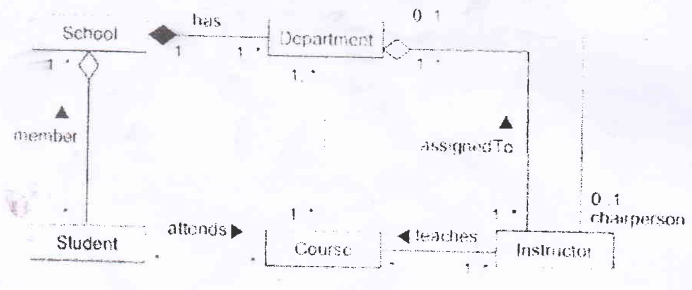
\includegraphics[width=5in]{images/oose_74_bh_2}

      \item Study the given case study and perform the followings: \hfill [2+8] (\bo{76 Bh})\\
        A travel agency wants an Airline Ticketing System to be developed for the office so that user can easily book flights tickets from anywhere. First of all, the customer enters the destination and date for the flight. After that, the system displays all the available airlines for the same along the route or available time which is provided by the airlines company. Now, the customer selects the airline which he/she finds appropriate where he/she can either book the ticket or confirm the ticket. The customer pays the ticket charge either via e-sewa or transferring the amount to the agency's bank account directly. The customer has to provide the valid email address to get the notification of booking or ticket confirmation.\\
        \enter a. List the conceptual classes.
        \enter b. Draw the complete Design Class Diagram using the listed conceptual classes. 
        \enter c. Convert class diagram to code by using any OOP language of your choice. \hfill [8] (\bo{76 Bh})

      \item (Assumed) Implement the design in the question: \hfill [6] (\bo{80 Ch})\\
        For an online doctor consultation enabling patients to register, log in, upload and save medical reports. Upon successful completion of the above actions, he/she can engage with doctor for personalized insights. \hfill [6] (\bo{80 Ch})

      \item Identify the different classes, relationships and draw a class diagram for ``Research Proposal Management System" as following: \hfill [8] (\bo{79 Ch})\\
        You need to create an IS that will manage information regarding research proposal submitted by university researchers to research funds (i.e., organizations funding academic research). The system will serve the Research Contracts division of the university researchers and the researchers. A researcher belongs to a department and occasionally submits research proposals. A research proposal has a title given to it by the researcher, but since a title may not be unique, the university's Research Contracts division assigns each proposal a unique research code. The proposal is submitted to a research fund (identified by a fund name). When a proposal is first submitted, the PIs specify how many years the research is supposed to take (between 1 to 4 years), and for every year they specify; how much money they request, who will be the coinvestigators (CIs) (ie., other university researchers who work on the research), and how many months will each of the CIs work on the research. The research fund may approve or disapprove the request, or approve a different amount of money. At the end of every year the PIs have to resubmit their request of funding for the next year, and the research fund may disapprove or approve any amount of money. The status, amount, and date of approval must be registered.
        \lb Also, implement the design class you have drawn with any suitable programming language. \hfill [8] (\bo{79 Ch})

      \item (Assumed) How can we create definition and methods from the design class diagram and interaction diagram? Explain with appropriate example. \hfill [6] (\bo{78 Ch})
     
    \end{enumerate}

  \subsection{Partitioning the analysis model}
    \begin{enumerate}
      \item Briefly explain partitioning the analysis model in system design process. \hfill [4] (\bo{\texttt{78 Ch}})
    \end{enumerate}

  \subsection{Concurrency and subsystem allocation}
    \begin{enumerate}
      \item Briefly explain the Concurrency and subsystem allocation in system design process. \hfill [4] (\texttt{82 Ka})
    \end{enumerate}

  \subsection{Task Management component}
  \subsection{Object DBMS}
    \begin{enumerate}
      \item What are the major features of object based DBMS? \hfill [2] (\texttt{79 Ash})

      \item How object based DBMS differs from RDBMS? \hfill [4] (\texttt{79 Ash})
    \end{enumerate}

  \subsection{Data Management components}
  \subsection{Resource Management components}
  \subsection{Inter sub-system communication}
  \subsection{Object Design process}

\pagebreak

\section{Object Oriented Testing}
  \begin{center} (6 Hours / 11 Marks) \end{center}

  \subsection{Overview of Testing and object oriented testing}
    \begin{enumerate}
      \item Why is software testing important? \hfill [2] (\bo{\texttt{81 Ch}})
        \lb Why testing is necessary in system development? \hfill [3] (\bo{\texttt{79 Ch}})

      \item How can you differentiate Software Verification and Validation? \hfill [2] (\texttt{80 Ash})

      \item Explain the different types of strategies is used in the different level of testing in object-oriented testing. \hfill [6] (\bo{\texttt{80 Ch}})

      \item How OO based testing differs from conventional type of software testing? \hfill [2] (\texttt{79 Ash})
    \end{enumerate}

  \subsection{Types of Testing}
    \begin{enumerate}
      \item Explain the different types of strategies used in OO Testing. \hfill [6] (\texttt{82 Ka})
    \end{enumerate}

    \subsubsection{Unit testing}
      \begin{enumerate}
        \item Define unit testing. \hfill [2] (\texttt{82 Ka})

        \item Explain how unit testing can be conducted in context of OO system development? \hfill [5] (\texttt{79 Ask})
      \end{enumerate}

    \subsubsection{Integrating testing}
      \begin{enumerate}
        \item Explain the different strategies for Integration Testing of OO system. \hfill [4] (\texttt{80 Ash})
      \end{enumerate}

    \subsubsection{System testing}
    \subsubsection{Thread Based testing}
      \begin{enumerate}
        \item Briefly describe thread based testing. \hfill [2] (\bo{\texttt{81 Ch}})
      \end{enumerate}

    \subsubsection{Use Based testing}
      \begin{enumerate}
        \item Briefly describe use based testing. \hfill [2] (\bo{\texttt{81 Ch}})

        \item Differentiate between thread-based testing and use-based testing. \hfill [4] (\bo{\texttt{79 Ch}})
      \end{enumerate}

  \subsection{Object oriented testing strategies}
    \begin{enumerate}
      \item What are the basic OO testing strategies? \hfill [4] (\bo{\texttt{78 Ch}})
    \end{enumerate}

  \subsection{Test case design for OO Software}
    \begin{enumerate}
      \item List out the overall approaches for designing Object Oriented Test Case. \hfill [4] (\bo{\texttt{78 Ch}})
    \end{enumerate}

  \subsection{Inter class test case design}
    \begin{enumerate}
      \item Write short notes on: Inter-class test case design. \hfill [3] (\bo{\texttt{81 Ch}})
        
      \item What are the steps to generate multiple class random test curves? Explain. \hfill [4] (\bo{\texttt{79 Ch}})

      \item Write short notes on: Multiple class testing. \hfill [4] (\bo{79 Ch})
    \end{enumerate}

\pagebreak

\section{Managing Object Oriented Software Engineering}
  \begin{center} (5 Hours / 9 Marks) \end{center}
  
  \subsection{Project selection and preparation}
    \begin{enumerate}
      \item What are the factors to be considered while selecting the first project in OOSE? Explain. \hfill [4] (\texttt{80 Ash})
      \item What are the factors to be considered while selecting a project? \hfill [2] (\bo{\texttt{81 Ch, 79 Ch, 78 Ch}})
    \end{enumerate}

  \subsection{Project development, organization and management}
  \subsection{Software project planning and scheduling and techniques}
  \subsection{COCOMO model}
    \begin{enumerate}
      \item Why is the COCOMO model useful? \hfill [2] (\texttt{82 Ka})
      
      \item Explain the different types of COCOMO model. \hfill [6] (\texttt{82 Ka})

      \item Write short notes on: COCOMO Model. \hfill [4] (\bo{\texttt{80 Ch}})

      \item Calculate effort of a project, which is an organic project having a size of 48 KDLOC using COCOMO model. \hfill [3] (\texttt{80 Ash})

      \item How can we calculate the effort and duration of a project using COCOMO model? Explain with example. \hfill [6] (\bo{\texttt{81 Ch, 78 Ch}})
    \end{enumerate}

  \subsection{Risk management process}
    \begin{enumerate}
      \item Explain Risk management process with proper flow diagram.
        \lb How risk management process is carried out in OOSE? Explain. \hfill [4] (\texttt{80 Ash})

      \item What are the main process of risk analysis in software engineering? \hfill [5] (\bo{\texttt{81 Ch}})

      \item List any two examples of potential risk areas involved in OOSE projects and how we can manage them. \hfill [4] (\bo{\texttt{79 Ch}})

      \item What could be the possible risks in software development projects? \hfill [2] (\texttt{79 Ash})
    \end{enumerate}

  \subsection{Software quality assurance}
    \begin{enumerate}
      \item Define Software Quality Assurance (SQA). \hfill [1] (\bo{\texttt{80 Ch}})
        \lb Write short notes on: SQA. \hfill [4] (\bo{\texttt{78 Ch}}, \texttt{80 Ash})

      \item What are the various activities and tasks involved in SQA? Explain in briefly. \hfill [5] (\bo{\texttt{80 Ch}})
    \end{enumerate}
    
  \subsection{Software metrics}
    \begin{enumerate}
      \item Write short notes on: Software metrics. \hfill [4] (\texttt{80 Ash})
    \end{enumerate}

\pagebreak

\section{No idea where they're from}
  \begin{enumerate}
    \item Write short notes on: Dewey Decimal Numbering and its use in modeling. \hfill [3] (\bo{74 Bh})
    \item Write short notes on: Reverse engineering. \hfill [5] (\bo{77 Ch, 76 Bh})

    \item Prepare a comparitive note on forward versus reverse engineering with mentioning the merits, demerits and implementation challenges. \hfill [6] (\bo{74 Bh})

    \item Compare: Forward vs Reverse Engineering. \hfill [3] (73 Ma)

    \item What are the key components of collaboration diagram? \hfill [5] (\bo{77 Ch})

    \item Write short notes on: Collaboration diagram. \hfill [4] (\bo{76 Bh})

    \item Describe the importance of collaboration diagram while designing a system. \hfill [3] (\bo{77 Ch})

    \item Prepare a collaboration diagram for making a hotel reservation. \hfill [6] (76 Ba)

    \item Explain controller and polymorphism GRASP pattern with example. \hfill [6] (\bo{81 Ch})
    \lb Explain concepts of controller and polymorphism as per the definiton outlined from GRASP design pattern with illustration. \hfill [8] (73 Ma)

    \item Explain about information expert creater and polymorphism pattern defined by GRASP. \hfill [6] (\bo{79 Ch})

    \item Explain about information expert, creator, controller and polymorphosim design patterns defined by GRASP. \hfill [6] (\bo{78 Ch})

    \item explain the purpose and benefits of information Expert, Creator, Controller and Polymorphosim design patterns defined by GRASP. \hfill [6] (\bo{74 Bh})

    \item Describe the term design pattern? \hfill [1] (\bo{75 Bh})

    \item What are the different components of design patterns? \hfill [4] (\bo{79 Ch})

    \item Describe the term Design Pattern. \hfill [2] (\bo{78 Ch})

    \item Define design pattern and framework. \hfill [2] (76 Ba)

    \item What are the key benefit of using design patterns? \hfill [5] (\bo{77 Ch})
    
    \item Explain MVC design pattern with the help of suitable example. \hfill [3] (\bo{77 Ch})
    \lb Write short notes on: MC pattern. \hfill [3] (73 Ma)

    \item What are pattern based design and its benefits? Prepare illustrative notes on pattern based design. \hfill [6] (\bo{74 Bh})

    \item Write short notes on: Multiplicity in association. \hfill [3] (\bo{81 Ch})

    \item Justify the statement that ``Coupling and Cohesion are the two sides of a coin'' with example. \hfill [3] (\bo{74 Bh}) [5] (\bo{80 Ch})

    \item Describe the importance of system contract. \hfill [2] (\bo{77 Ch})

    \item What is operation contract? \hfill [2] (\bo{75 Bh})

    \item Describe pre-condition and post-condition of contract. \hfill [2] (\bo{77 Ch})

    \item Construct a system contract for any one system operation with respect to case study mentioned in [6] (\bo{77 Ch}) question of domain model. \hfill [4] (\bo{77 Ch})

    \item Write short notes on: Software building complexity and dealing strategy. \hfill [4] (76 Ba)

    \item Write short notes on: Business workflow based swim-lane. \hfill [4] (76 Ba)

    \item Write short notes on: Distributed system implementation issues. \hfill [4] (75 Ba)
  \end{enumerate}

\end{document}
